\chapter{基于华为云的课程实践}

本次课程项目基于华为云,需要完成一个自习室预定系统,
并利用华为云进行代码管理、持续集成和持续部署。
本文对本人编写的API设计,前端、后端、测试代码及华为云持续集成和持续部署模块进行介绍。

\section{项目框架}

项目分为前端和后端,前端使用Web技术栈,并通过Web API和后端进行通信。
后端使用RESTful风格设计通信接口,在服务器监听API请求,并与数据库通信进行信息的获取和存储。
同时,编写后端代码时同时编写相关单元测试用例,用于检查代码编写的正确性。

\section{代码构成}

\subsection{API设计}

\begin{figure}
    \centering
    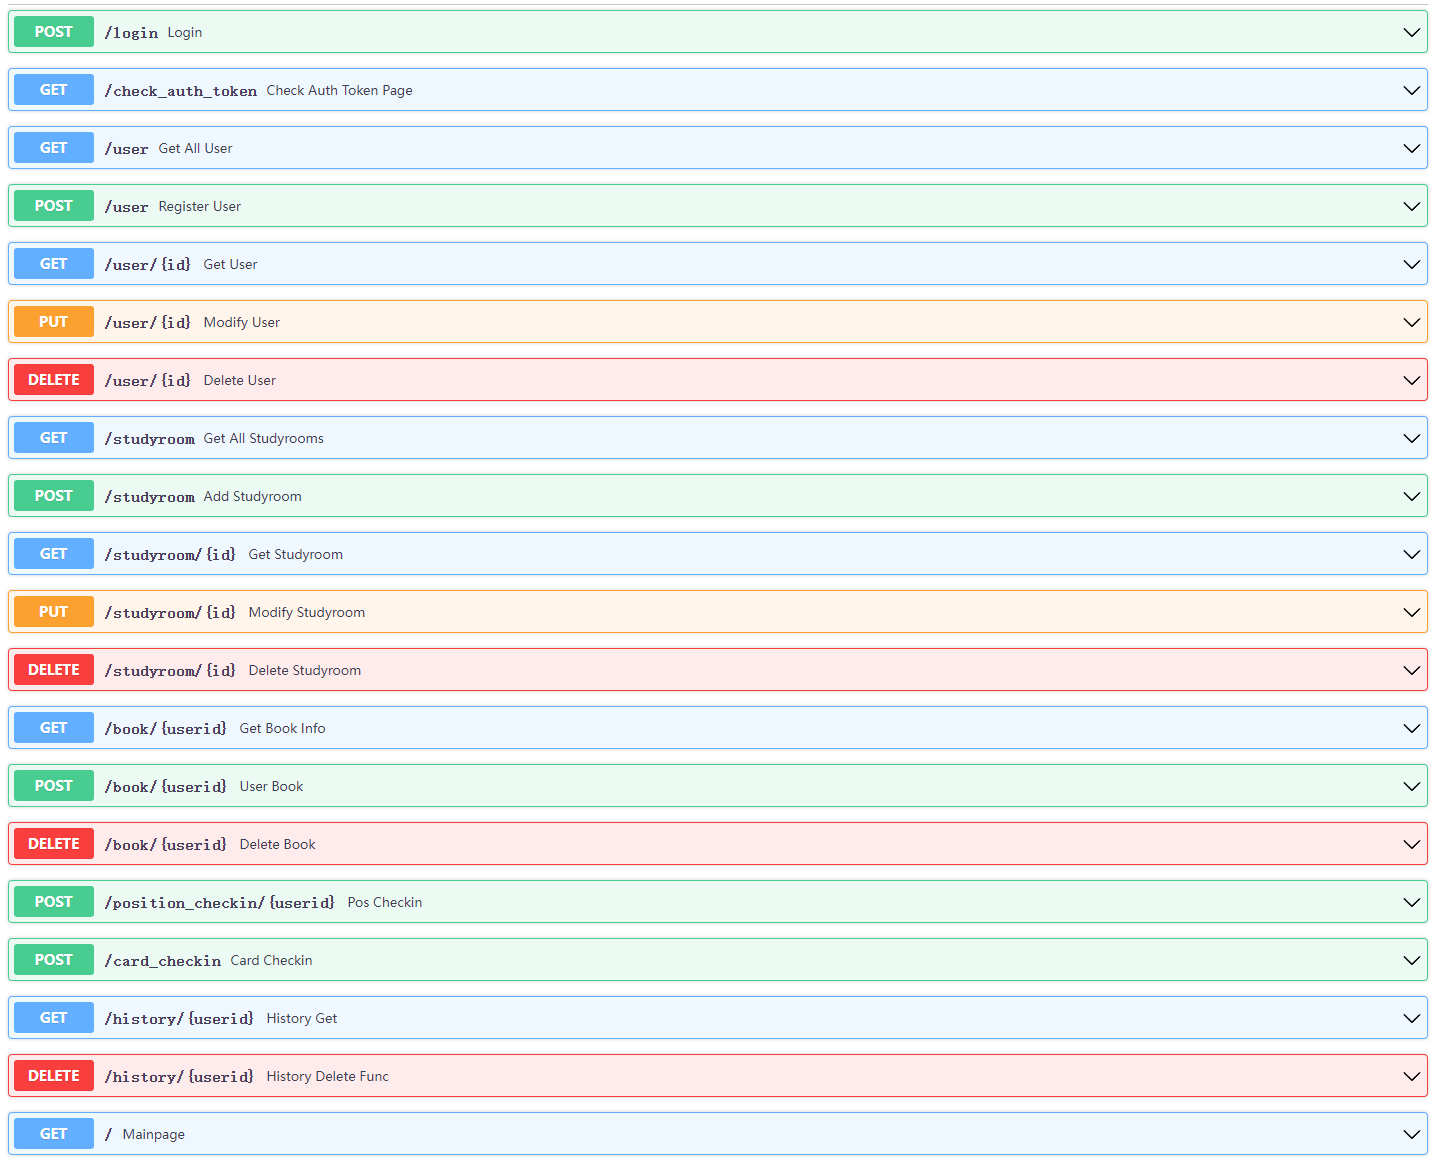
\includegraphics[width=\textwidth]{figures/project/API.png}
    \caption{通信API}
    \label{fig:project_api}
\end{figure}

如图\ref{fig:project_api}所示,项目使用RESTful思想设计API。除去用户注册和用户登录,其他API请求均需要携带Auth-Token标头
提供认证token,后端以此验证身份。API分为账户管理、自习室管理、预约管理、签到管理、历史管理五类,
可在后端代码介绍中看到。

\subsubsection{前端代码}

前端代码基于Vue 2.0框架,基于助教提供的脚手架。框架中以App.vue作为主页面,
包含了导航栏和通知模块,使用Vue Router功能完成非刷新的页间跳转。
图\ref{fig:project_admin_login}展示了管理员登录后的用户管理页面。

\begin{figure}
    \centering
    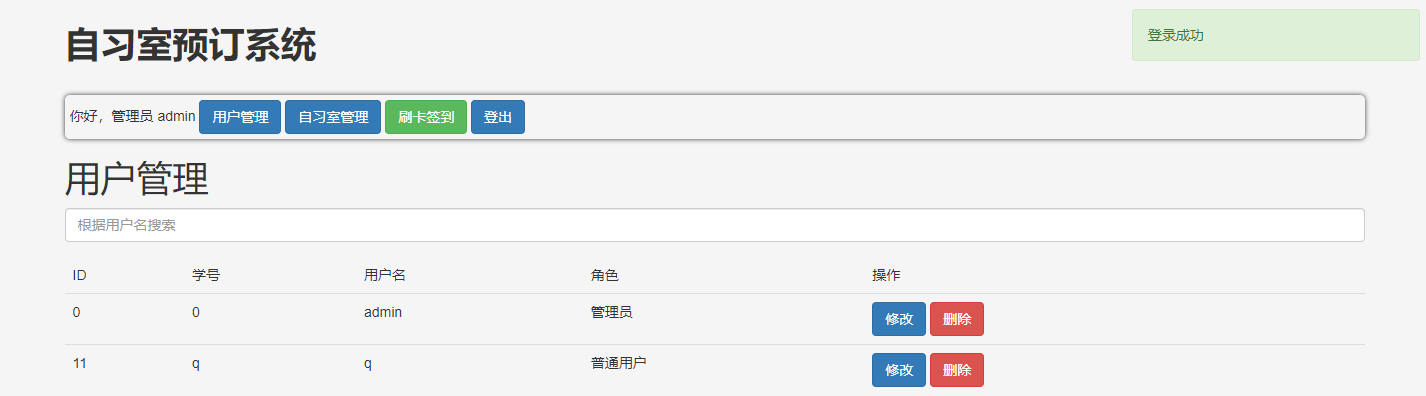
\includegraphics[width=\textwidth]{figures/project/frontend_admin_login.png}
    \caption{前端管理员账户登录页面}
    \label{fig:project_admin_login}
\end{figure}

其中导航栏根据当前的登录状态和不同用户身份会展示不同的功能按钮。
未登录时展示注册和登录按钮;普通用户登录后展示个人信息、签到、预约、历史、登出按钮;
管理员登录后展示用户管理、自习室管理、刷卡签到、登出按钮。

前端需要持久化维护的信息只有用户认证token、用户身份、用户ID和token过期时间,
这些信息会存于Vue Store和localStorage中。当首次加载页面发现token已经过期时,
前端会自动清除已有信息并返回登录页面。由于后端同样会对用户token及信息做验证,
因此在前端伪造持久化信息除了能够展示页面外没有办法获取数据。

页面间进行信息传递使用Vue Store。除了上述身份和认证信息外,仅提示信息(右上角成功提示)
需要传递,主页面加载提示框控件后,控件绑定store中提醒内容,当收到提醒后会自动渲染
最近5秒内的提醒。其他信息均在访问时向后端请求,减少信息泄漏。

\subsection{后端代码}

\begin{figure}
    \centering
    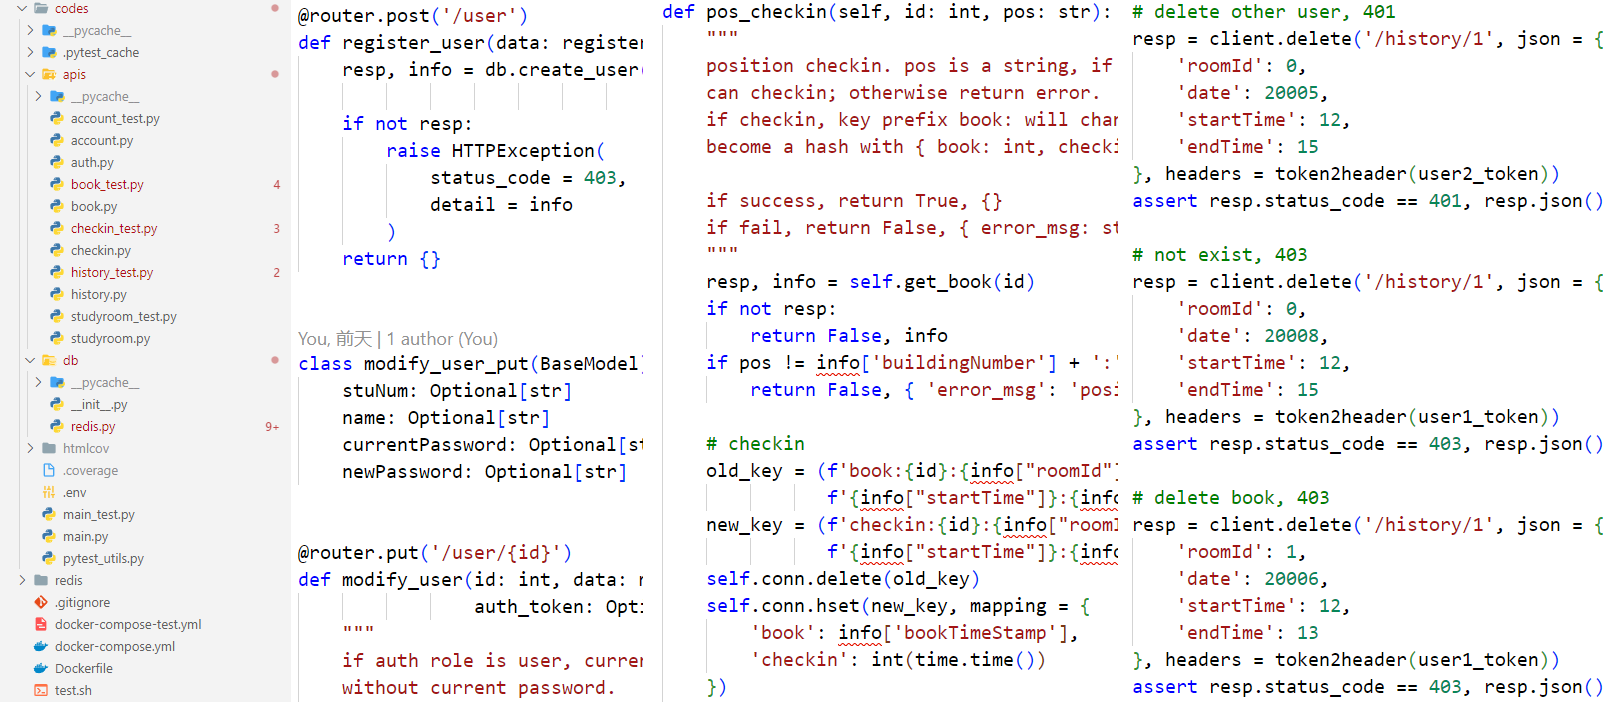
\includegraphics[width=\textwidth]{figures/project/backend_code.png}
    \caption{后端代码结构,及后端,数据库和测试代码片段}
    \label{fig:project_backend_code}
\end{figure}

\begin{figure}
    \centering
    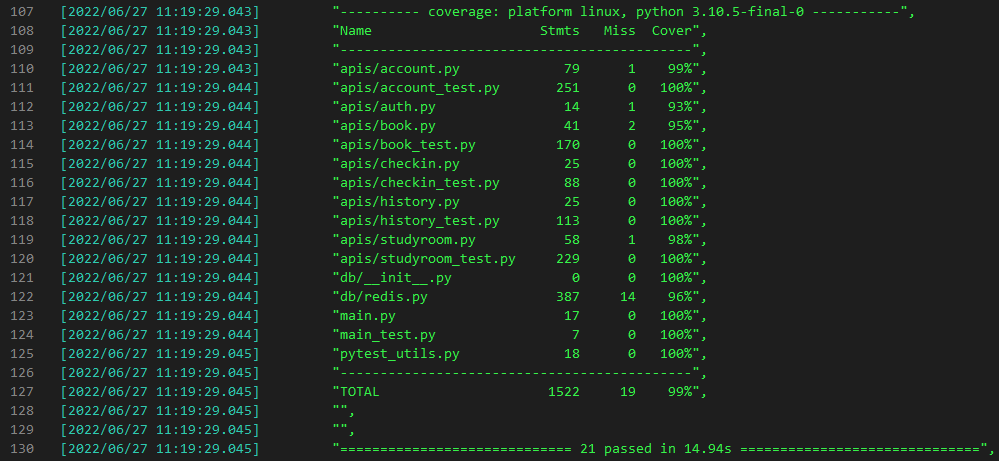
\includegraphics[width=\textwidth]{figures/project/coverage.png}
    \caption{后端代码coverage测试结果}
    \label{fig:project_coverage}
\end{figure}

图中展示了后端代码的结构,以及从左往右分别为后端、数据库操作和测试的部分代码片段。
后端代码使用Python FastAPI框架,并使用PyTest编写单元测试,coverage检查代码覆盖率。
根据API设计中所提到的,将API分为五大类,每类包含一个文件。同时,对每个文件编写了
一个单元测试文件,包含若干测试用例,测试基于API,检查返回值和返回数据是否正确。
同时,coverage也会检查代码的覆盖率,用于观察是否有代码漏写测试用例。
图\ref{fig:project_coverage}中展示了一次持续集成中coverage的代码覆盖率,其中未覆盖代码均为函数调用时一些异常情况的冗余判断,
由于之前调用函数时已经包含相关判断,因此该判断永远不成立。其余逻辑代码均实现了测试的全覆盖。

数据库部分,目前使用了轻量级数据库redis。由于使用类进行数据库操作,
因此写在了一个文件中。设计时准备将数据库类设计为单类,
但由于分析后发现当前数据库非单类也能正常工作,就未实现单类模式。

由于使用类包装了数据库访问接口,因此后端不关心数据库的实际实现,
只要接口保持一致,可以很方便的切换为其他数据库。
同时,当前数据库未根据API分类进行拆分,且和后端代码耦合。实际中可以将后端独立出来,
作为另一个服务,后端通过服务接口访问数据库,这样可以更加降低耦合度。
如果将数据库相关代码剥离,由于各类API之间互不关联,该后端代码也可以很容易的改造为微服务架构。

Redis作为轻量级键值对数据库,具有很高的吞吐性能,一般作为内存数据库和缓存数据库使用。
在本项目中,由于需要存储的数据种类较少,且相互依赖关系较为简单(仅预定座位时,预定操作
会依赖于用户和自习室),为了开发简便,未使用关系型数据库。实际项目中,
对于有较为复杂的依赖关系的情形,使用关系型数据库可以减少依赖关系出错的情况。

\section{华为云持续集成和持续部署}

由于前端和后端分别为两个代码仓库,采用了两条CI+CD流水线,
如图\ref{fig:huawei_pipeline}所示。由于Docker部署的简便性,前端和后端均使用Docker
进行部署,其中后端的Python和数据库环境分离,由两个container构成,使用docker-compose统一部署
和通信,并仅暴露FastAPI的接口可供外部访问,因此内部redis数据库无需进行身份验证,
减少工作量。

在前端代码的CI+CD中,首先会利用华为云的编译构建功能,使用NodeJS构建前端代码。
然后基于Nginx镜像,将编译完成后的代码复制到镜像中,同时编写Nginx配置,
将编译完成的静态网页配置访问。之后,将该镜像打包上传至华为云的镜像管理,
用于之后部署。在部署阶段,华为云会通过主机组的SSH访问本组使用的服务器,
停止当前运行的容器,拉取最新版本的镜像,并使用最新镜像重新启动容器。

在后端代码的CI+CD中,由于华为云的构建和测试功能不够定制化,
使用测试部署的方式进行。由于基于docker-compose的方式,进行测试部署非常容易。
同时只需在测试时将启动FastAPI换为执行pytest,测试时不会暴露接口,数据库也新启动一个
独立数据库, 在同一台服务器上执行测试完全不会影响
该服务器上已运行的线上服务。这更加体现了使用容器技术的优越性。
后端代码提交后会先进行测试部署,此时会使用pytest检查后端代码是否能够通过
所有测试用例,并给出代码覆盖率的报告。如果代码通过了测试,
则会进行代码部署,通过SSH连接服务器,停止当前运行的docker,拉取最近代码,
重新构建镜像并启动新实例。

经过上述流水线的配置,对于前端和后端代码,仅需要直接推送代码至代码库,
流水线就会自动对代码进行持续集成,并在通过编译和测试后自动部署到服务器上,全程
不需要人工干预。在持续集成失败后对线上服务不会造成影响,在持续集成通过后
线上服务仅会在停止并重新启动实例时断线不到10秒,并在之后无缝升级。

\section{实践中遇到的困难和体会}

在使用华为云进行CI和CD时,也碰到了很多困难。本节中会对碰到的一些困难和体会进行总结。

\subsection{权限和认证问题}

该问题出现在流水线阶段。首先是流水线由本人搭建,因此测试时没有发现流水线有执行权限的问题。
虽然将流水线设置为了任意用户均可执行,但是其中涉及到镜像的推送,由于推送到的镜像
仓库的owner是我自己,因此我可以直接推送,而别人不行。虽然之后修改了推送权限,
但是由于组员都不开发了所以未测试是否修改成功。

另一个认证问题则来自于认证Token。华为云中通过填写认证Token对镜像进行推送认证,
然而在示例代码中Token的时效只有24小时。这导致了最开始可以执行的流水线一天以后
推送失败。解决方法是重新生成一个有效期是永久的Token。华为云在这里做的很不便利,
需要手动用华为云的CLI创建生成永久期限Token。

\subsection{Compose的测试和部署}

华为云的流水线套件中没有直接支持docker-compose的多容器部署的操作,
由于后端和数据库是两个容器,测试了很多种方式最后都失败了,
最后选择了直接测试部署到服务器上的方式完成CI流水线。相比而言
GitHub Actions中可进行的操作更多,环境更完整,这个方面华为云需要改进。

\subsection{Podman和Docker}

在提供的华为云服务器中,使用了Podman代替了Docker。一般情况下不会有问题,
但是在使用compose部署时仍然碰到了一些麻烦,最后通过在服务器上保存两份后端代码,
一份用于生产环境部署,一份用于测试部署解决该问题。当然,在实际情况下,不需要
在同一台服务器上共享,不会碰到类似问题。

\subsection{前端的本地调试}

前端需要搭配后端才能使用,目前的前端使用XMLHttpRequest直接访问硬编码的服务器地址,
因此进行前端调试时访问的是生产环境的数据库,这种做法会改动生产环境,不能完整测试,
且不发版无法修改后端地址。更合适的方法可能是将其作为配置变量之一,在开发调试时可以定向至
测试用后端和服务器,从而避免影响线上服务。

\subsection{跨域资源共享}

由于目前是前后端分离,且前端通过XMLHttpRequest异步和服务器通信,两者运行的端口不同,
导致了出现跨域资源共享(CORS)的问题。此时需要对FastAPI增加跨域资源访问配置插件,
允许指定域名的访问。本项目中为了简便且本地测试和生产环境均能够执行,
将允许跨域设置为全部允许。